Let's make this concrete with a specific process: the "Golden Mean".
This process generates binary sequences (0s and 1s) with a specific rule:
\begin{center}
    \textit{"No two consecutive 0s are allowed."}
\end{center}
If we see a $0$, the next symbol \textit{must} be a $1$. If we see a $1$, the next symbol can be $0$ or $1$ (with equal probability, say).

\begin{sidebar}{Why ``Golden Mean''?}
The name comes from the growth rate of the number of allowed sequences. The number of valid binary strings $N(L)$ of length $L$ containing no ``00'' follows the Fibonacci sequence. For large $L$, $N(L)$ grows as $\phi^L$, where $\phi = \frac{1+\sqrt{5}}{2} \approx 1.618$ is the Golden Ratio.
\end{sidebar}

\subsection{Inferring the Structure}
We run the CSSR algorithm (Causal State Splitting Reconstruction) on a generated sequence of 100,000 symbols. The algorithm looks at the statistics of subsequences and groups histories that lead to similar future probabilities.

\begin{emiclisting}[label=lst:pipeline]{The Pipeline}
\begin{lstlisting}[language=Python, basicstyle=\tiny\ttfamily, numbers=none]
from emic.sources import GoldenMeanSource
from emic.sources.transforms import TakeN
from emic.inference import CSSR, CSSRConfig
from emic.analysis import analyze

# 1. Define the source
source = GoldenMeanSource(p=0.5)

# 2. Configure the algorithm
cssr = CSSR(CSSRConfig(max_history=10))

# 3. The Inference Pipeline
# Source >> Transform >> Algorithm
result = source >> TakeN(100000) >> cssr

# 4. Analysis
summary = analyze(result.machine)
print(f"States: {summary.num_states}")
print(f"C_mu: {summary.statistical_complexity:.2f} bits")
\end{lstlisting}
\end{emiclisting}

\begin{emicfigure}[label=fig:gm_machine]{The $\epsilon$-machine for the Golden Mean Process.}
    \centering
    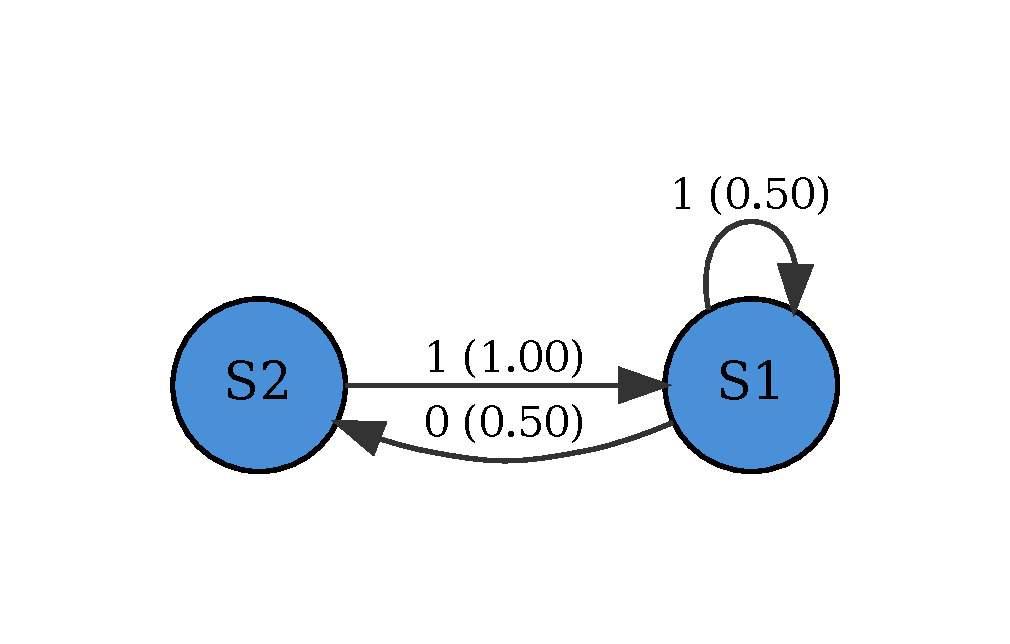
\includegraphics[width=\columnwidth]{figures/golden_mean_machine.pdf}
\end{emicfigure}

\subsection{Reading the Machine}
Look at the graph in Figure \ref{fig:gm_machine}.
\begin{itemize}
    \item \textbf{States}: There are two states. Let's call them $A$ and $B$.
    \item \textbf{Transitions}:
    \begin{itemize}
        \item From $A$, we can see '1' (loop back to $A$) or '0' (go to $B$).
        \item From $B$, we \textit{only} see '1' (and go back to $A$).
    \end{itemize}
\end{itemize}

Wait, does this match our rule?
\begin{itemize}
    \item State $A$ represents the condition "Last symbol was a 1". Since the last symbol was 1, we are free to emit 0 or 1 next.
    \item State $B$ represents the condition "Last symbol was a 0". Since the last symbol was 0, the rule says we \textit{must} emit a 1. So there is only one arrow leaving $B$.
\end{itemize}

The $\epsilon$-machine has automatically discovered the "No 00" rule just from the data! It identified that "histories ending in 0" have different predictive consequences than "histories ending in 1".
